% Abyss 技术报告：在两张显卡上分层运行 DeepSeek-V4.1-Flash
% 编译：tectonic -X compile report.tex（字体用 macOS 自带的 Palatino、宋体和 Helvetica Neue）
\documentclass[11pt,a4paper]{article}

\usepackage[a4paper,top=2.6cm,bottom=2.6cm,left=2.7cm,right=2.7cm]{geometry}
\usepackage{fontspec}
\usepackage{xeCJK}
\setmainfont{Palatino}
\setsansfont{Helvetica Neue}
\setmonofont{Menlo}[Scale=0.82]
\setCJKmainfont[BoldFont={Songti SC Bold}]{Songti SC}
\setCJKsansfont{Songti SC}
\setCJKmonofont{Songti SC}
\linespread{1.3}
\setlength{\emergencystretch}{2em}

\usepackage{amsmath}
\usepackage{graphicx}
\usepackage{booktabs}
\usepackage{tabularx}
\usepackage{array}
\usepackage{multirow}
\usepackage{xcolor}
\usepackage{enumitem}
\usepackage{caption}
\usepackage{subcaption}
\usepackage{tikz}
\usepackage{pgfplots}
\pgfplotsset{compat=1.18}
\usepackage{hyperref}
\hypersetup{colorlinks=true,linkcolor=dsblue,citecolor=dsblue,urlcolor=dsblue}

\definecolor{dsblue}{HTML}{4D6BFE}
\definecolor{dsviolet}{HTML}{8E7CF0}
\definecolor{dslight}{HTML}{C9D3FF}
\definecolor{dsgray}{HTML}{B8BCC8}
\definecolor{dsdark}{HTML}{1E2A5A}
\definecolor{dsorange}{HTML}{F29A4A}

\DeclareCaptionLabelSeparator{bar}{\ |\ }
\captionsetup{labelsep=bar,font=small,justification=justified,singlelinecheck=false}
\captionsetup[sub]{labelformat=parens,labelsep=space,justification=centering}
\renewcommand{\figurename}{图}
\renewcommand{\tablename}{表}
\renewcommand{\contentsname}{目录}
\renewcommand{\refname}{参考资料}
\renewcommand{\appendixname}{附录}

\setlist{itemsep=0.2em,topsep=0.4em}
\newcommand{\code}[1]{\texttt{#1}}
\newcommand{\tps}{tok/s}

\pgfplotsset{
  abyss/.style={
    axis lines*=left,
    ymajorgrids,
    grid style={dsgray!40},
    tick label style={font=\footnotesize},
    label style={font=\footnotesize},
    legend style={font=\footnotesize,draw=none,fill=none},
    every axis plot/.append style={line width=0.6pt},
  },
}

\begin{document}

% ---------------------------------------------------------------- title page
\thispagestyle{empty}
\noindent

\begin{tikzpicture}[baseline=(t.base)]
  \fill[dsblue] (0,0) rectangle (0.62,0.62);
  \draw[white,line width=1.4pt,line cap=round] (0.10,0.36) .. controls (0.20,0.48) and (0.26,0.48) .. (0.31,0.36) .. controls (0.36,0.24) and (0.42,0.24) .. (0.52,0.36);
  \draw[white!70!dsblue,line width=1.1pt,line cap=round] (0.10,0.20) .. controls (0.20,0.30) and (0.26,0.30) .. (0.31,0.20) .. controls (0.36,0.10) and (0.42,0.10) .. (0.52,0.20);
  \node[anchor=west,inner sep=0] (t) at (0.80,0.31) {\sffamily\bfseries\Large\color{dsblue}abyss};
\end{tikzpicture}

\vspace{0.6em}
\begin{center}
  {\LARGE\bfseries Abyss：在两张显卡上分层运行\\[0.25em] DeepSeek-V4.1-Flash}\\[1.0em]
  {\large Abyss}\\[0.2em]
  {\small 2026 年 10 月}
\end{center}

\vspace{0.4em}
\begin{center}{\large\bfseries 摘要}\end{center}
\vspace{-0.3em}
\noindent
长上下文智能体把推理的压力从算力推到了显存、内存和 PCIe 上。DeepSeek-V4.1-Flash 总参数 763B，原生权重约 474 GiB，超过一台双卡工作站（2 × RTX PRO 6000 Max-Q，显存合计 191 GiB；内存 192 GB）的全部容量。我们在 mx-llama.cpp 上实现了一个分层推理调度器 Abyss：编码器各层的专家常驻显存，解码器后 18 层的专家放在主机内存，由 GPU 上的专家缓存和 CPU 分担，Engram 大表留在 NVMe。围绕这款模型的编码器-解码器结构（CED）、压缩注意力和稀疏索引器，我们依次实现了 CED 感知预填充、Engram 预取、官方稀疏索引器、解码注意力的 top-k 收集、按热度准入的专家缓存未命中分流、预填充大批次的 CPU 分流，以及让提示词末段一遍算完的调用合并，最后把内存从 3600 MT/s 提到 5200 MT/s。在保持原生 MXFP4 精度的前提下（每项改动对改动前的 KLD 都在数值底线以内），预填充的提升最大：4.8 万 token 提示词从 135 s（355 \tps{}）降到 22.7 s（2,111 \tps{}），快约 6 倍，其中 CED 感知预填充把解码器层的计算量从约 96 万个「token × 层」降到约 2.4 万个，贡献最大；Engram 页缓存冷时，预取把冷读开销从约 39 s 降到约 2 s；多轮智能体会话里，之后每轮（1,200--1,600 token）的预填充从 5.7--7.2 s 降到 2.7--3.2 s。解码从 4.8 万上下文的 14.1 \tps{} 提升到只追加的多轮会话里的 31--33 \tps{}，4.8 万和 9.6 万上下文一样；剩下的时间主要花在把未命中的专家从内存经 PCIe 搬到 GPU。我们同时记录了评估方法（两档数值底线、对官方实现的单层对拍、逐 token 剖析）、一个让解码速度虚高的测法陷阱，以及在真实 Codex 负载中发现并修复的缺陷。

\vspace{0.2em}
\begin{figure}[!h]
  \centering
  \begin{subfigure}[b]{0.49\textwidth}
    \centering
    \begin{tikzpicture}
      \begin{axis}[abyss,
        width=\linewidth, height=4.0cm,
        ybar, bar width=12pt, ymin=0, ymax=42,
        ylabel={解码速度（\tps）},
        xtick={1,2,3,4,5,6},
        xticklabels={原版, 专家缓存, 稀疏索引器, 注意力取 top-k, 未命中分流, 多轮会话实测},
        xticklabel style={font=\scriptsize,align=center,text width=1.1cm},
        nodes near coords, nodes near coords style={font=\scriptsize},
        enlarge x limits=0.12]
        \addplot[fill=dslight,draw=dsblue] coordinates {(1,14.1) (2,25.2) (3,27.7) (4,30.6) (5,36.1)};
        \addplot[fill=dsblue,draw=dsblue,bar shift=0pt] coordinates {(6,31.8)};
      \end{axis}
    \end{tikzpicture}
    \caption{}
  \end{subfigure}\hfill
  \begin{subfigure}[b]{0.49\textwidth}
    \centering
    \begin{tikzpicture}
      \begin{axis}[abyss,
        width=\linewidth, height=4.0cm,
        ybar, bar width=17pt, ymin=0, ymax=150,
        ylabel={预填充时间（s）},
        xtick={1,2,3,4},
        xticklabels={原版, CED（FFN）, CED（注意力）, 稀疏索引器},
        xticklabel style={font=\scriptsize,align=center,text width=1.4cm},
        nodes near coords, nodes near coords style={font=\scriptsize},
        enlarge x limits=0.18]
        \addplot[fill=dslight,draw=dsblue] coordinates {(1,135) (2,41.8) (3,27.9)};
        \addplot[fill=dsblue,draw=dsblue,bar shift=0pt] coordinates {(4,22.7)};
      \end{axis}
    \end{tikzpicture}
    \caption{}
  \end{subfigure}
  \caption{(a) 4.8 万上下文的单流解码速度，依次叠加各项优化（第 4 节）；第 3--5 根是同一提示词第二次生成，缓存命中偏高；最后一根是只追加的多轮会话实测（9.6 万上下文、内存 5200 MT/s，\S\ref{sec:realdecode}）。(b) 4.8 万 token 提示词的预填充时间，Engram 页缓存已热（第 5 节）。}
  \label{fig:hero}
\end{figure}

\newpage
\tableofcontents
\newpage

% ---------------------------------------------------------------- 1
\section{引言}

智能体把大模型的典型请求从「短问短答」变成了「长上下文、多轮、带工具调用」。一个编程智能体每一轮都要在几万 token 的上下文后面追加回复、工具结果或追问，再让模型继续生成。这种负载有两个特点：一是上下文长，注意力和 KV 的开销随之增长；二是每一轮新增的内容不多，但首 token 之前的那段预填充决定了用户等待的时间。

DeepSeek-V4.1-Flash~\cite{v41} 是为这类负载设计的。它有 552B 主干参数、196.6B 的 Engram 查表和约 14B 的 DSpark 草稿模型；40 层中前 20 层是因果编码器、后 20 层是解码器（CED），提示词的每个 token 只需走完编码器，生成的 token 才走完全部 40 层；注意力把 KV 按 2 倍或 1 倍压缩，再由稀疏索引器为每个查询挑出 512 个压缩位置；路由专家 384 个，每个 token 选 6 个，权重是原生 MXFP4。

问题在于容量。原生权重约 474 GiB（专家 268.9 GiB，Engram 189 GiB），而我们的机器只有两张 RTX PRO 6000 Max-Q（每张 95.6 GiB）和 192 GB 内存，合计约 383 GiB。公开的双卡方案~\cite{diffbot} 把专家量化到 3.0 bpw，速度很快（同样两张 RTX PRO 6000，单流解码 66--74 \tps{}，4.6 万 token 提示词预填充约 1 万 \tps{}），但相对原版的 KL 散度为 0.0545、top-1 一致率 92.9\%，而且需要约 250 GiB 空闲内存，本机放不下。我们选择了另一条路：保留原生 MXFP4，把权重按热度分布在显存、内存和 NVMe 三层（方案 B），在 mx-llama.cpp~\cite{mxllama} 上实现调度器 Abyss，再逐项找出瓶颈并优化。

本报告记录这一过程。主要结果见表~\ref{tab:summary}：

\begin{itemize}
  \item \textbf{解码}：GPU 专家缓存、解码注意力只取 top-k 行、按热度准入的未命中分流，使解码从 14.1 \tps{} 提升到只追加的多轮会话里约 30 \tps{}（内存 3600 MT/s），4.8 万和 9.6 万上下文一样；内存提到 5200 MT/s 后为 31--33 \tps{}。
  \item \textbf{预填充}：CED 感知预填充让解码器层只计算后面还能看到的 token，加上 Engram 预取和官方稀疏索引器，4.8 万 token 提示词从 135 s 降到 22.7 s；大批次分流和末段一遍算完再把多轮会话每轮的预填充从 5.7--7.2 s 降到 2.9--3.5 s。
  \item \textbf{测法}：同一提示词第二次、一字不差的生成会让专家缓存命中偏高，解码速度虚高约 15--20\%。我们用只追加的多轮会话重新测量，并据此修正了此前的结论。
  \item \textbf{正确性}：所有改动都有对拍。我们区分了两档数值底线，并对稀疏索引器和解码注意力做了对官方 PyTorch 实现、对 float64 的逐层对拍。
  \item \textbf{真实负载}：在 Codex 的实际请求中发现了 prompt 缓存的选择问题和三处只在特定提示词长度下出现的崩溃，均已修复。
\end{itemize}

\begin{table}[t]
  \centering
  \small
  \caption{各阶段的改动与效果。解码在 4.8 万上下文下测；预填充为 4.8 万 token 提示词、Engram 页缓存已热；KLD 是对改动前的 logits，「—」表示没有改变数值。}
  \label{tab:summary}
  \begin{tabularx}{\textwidth}{@{}l X l l@{}}
    \toprule
    补丁 & 改动 & 效果 & 对拍 \\
    \midrule
    环境变量 & 预填充的 MXFP4 矩阵乘改用 8 bit 激活（W4A8） & 预填充约慢 5\% & 0.044 $\to$ 0.012\textsuperscript{*} \\
    分支自带 & GPU1 上的专家缓存（14 GB，约 780 槽位，LRU） & 解码 14.1 $\to$ 25.2 \tps{} & 0.0005 \\
    0003 & CED 感知预填充：解码器层只算可见 token 的 FFN & 预填充 135 $\to$ 41.8 s & 0.00004 \\
    0004 & Engram 整批预取 & 冷缓存 91.1 $\to$ 54.3 s & — \\
    0005 & 解码器层的注意力也只算子集 & 41.8 $\to$ 27.9 s & 0.00007 \\
    0006 & 补上官方稀疏索引器（top-512） & 27.9 $\to$ 22.7 s；修正长上下文 & 见 \S\ref{sec:indexer} \\
    0008 & 解码注意力只取 top-k 行 & 解码 27.7 $\to$ 30.6 \tps{}\textsuperscript{‡} & 0.003\textsuperscript{†} \\
    0009 & 未命中按热度一半上传、一半交给 CPU & 30.6 $\to$ 36.1 \tps{}\textsuperscript{‡} & 0.0003\textsuperscript{†} \\
    0014 & 预填充大批次分流 & 每轮 5.7--7.2 $\to$ 4.6--5.6 s & 0.0005 \\
    0015 & 提示词末段一遍算完：末段不拆调用，最后一个 ubatch 对齐到满 & 每轮 4.6--5.6 $\to$ 2.9--3.5 s & 0.009\textsuperscript{§} \\
    BIOS & 内存 3600 $\to$ 5200 MT/s & 解码约 +6\%，每轮 2.7--3.2 s & 重跑一致 \\
    \bottomrule
  \end{tabularx}
  \par\smallskip\raggedright\footnotesize *\ 预填充路径对解码路径的 KLD，不是对改动前。†\ server 上 temperature 0 生成时的 top-20 KL；0008 经过编码器层，属于较高的一档底线（\S\ref{sec:floors}）。‡\ 同一提示词第二次、一字不差的生成，缓存命中偏高；只追加的多轮会话见 \S\ref{sec:realdecode}。§\ 和只换 ubatch 大小的差别一样（\S\ref{sec:tailmerge}）。
\end{table}

% ---------------------------------------------------------------- 2
\section{硬件与模型}

\subsection{硬件}

表~\ref{tab:hw} 是机器的配置和实测带宽。两点决定了后面的设计：内存是双通道、每通道两条，优化过程中运行在 3600 MT/s，纯读只有约 44 GB/s（最后提到 5200 MT/s，见第 7 节）；两张卡各走 PCIe 5.0 x8，单卡主机到显存约 28.9 GB/s，但两卡同时从主机读合计只有 43.4 GB/s，被内存带宽卡住。所以无论专家由 CPU 计算还是上传到 GPU，每读一个专家都要占用同一份内存带宽。

\begin{table}[h]
  \centering
  \small
  \caption{硬件与实测带宽（2026-10-20，STREAM 与 nvbandwidth；括号里是 2026-10-25 内存提到 5200 MT/s 后的值）。}
  \label{tab:hw}
  \begin{tabularx}{\textwidth}{@{}l X@{}}
    \toprule
    项目 & 配置与实测 \\
    \midrule
    GPU & 2 × RTX PRO 6000 Blackwell Max-Q（300 W），每张 97,887 MiB GDDR7，SM120 \\
    互联 & PCIe 5.0 x8 / x8，P2P 经 CPU，无 NVLink；卡间单向约 27.7 GB/s \\
    CPU & AMD Ryzen 9 9950X，16 核 32 线程，单 NUMA \\
    内存 & 4 × 48 GB DDR5（双 rank），双通道 2DPC，3600 MT/s；纯读 44 GB/s，STREAM Copy 42 / Triad 32 GB/s（5200 MT/s：54、53.5 / 39.7） \\
    主机 $\to$ 显存 & 单卡 28.9 GB/s；两卡同时合计 43.4 GB/s（5200 MT/s：50.6） \\
    存储 & Samsung 9100 PRO 4TB（PCIe 5.0）、990 PRO 4TB（PCIe 4.0） \\
    \bottomrule
  \end{tabularx}
\end{table}

\subsection{模型}

图~\ref{fig:arch} 是 DeepSeek-V4.1-Flash 的逐层结构和方案 B 在本机的布局，维度取自 GGUF 元数据。与本报告相关的结构特点有四个：

\begin{itemize}
  \item \textbf{编码器-解码器（CED）}。第 0--19 层是因果编码器，第 20 层的压缩器生成所有解码器层共享的全局 KV。解码器层只通过各自 128 个 token 的滑动窗口读自己的隐状态，因此提示词前面的大部分 token 不需要走完解码器。
  \item \textbf{压缩注意力}。第 0--1 层只有滑动窗口；第 2--19 层把每 2 个 token 压成一行，第 20--39 层每个 token 一行。压缩 KV 只在第 2、8、14、20 层写入，其后的层复用。每个查询有 64 个头，键值只有 1 个 512 维的头（K = V）。
  \item \textbf{稀疏索引器}。第 2、8、14、20、24、28、32、36 层用 32 个头、128 维、FP4 的查询和键给压缩位置打分，选出 top-512；第 20 层还按每 8 行一块挑出 2,048 个候选块，供第 24--36 层重选。其余层沿用最近索引源的结果。
  \item \textbf{专家与 Engram}。每层 384 个路由专家选 6 个，外加 1 个共享专家；每个 MXFP4 专家约 18.8 MB，每层 7.2 GB。第 1、14 层按最近 2--4 个 token 的 n-gram 哈希查两张约 3.84 亿行的大表。
\end{itemize}

\begin{figure}[p]
  \centering
  \makebox[\textwidth][c]{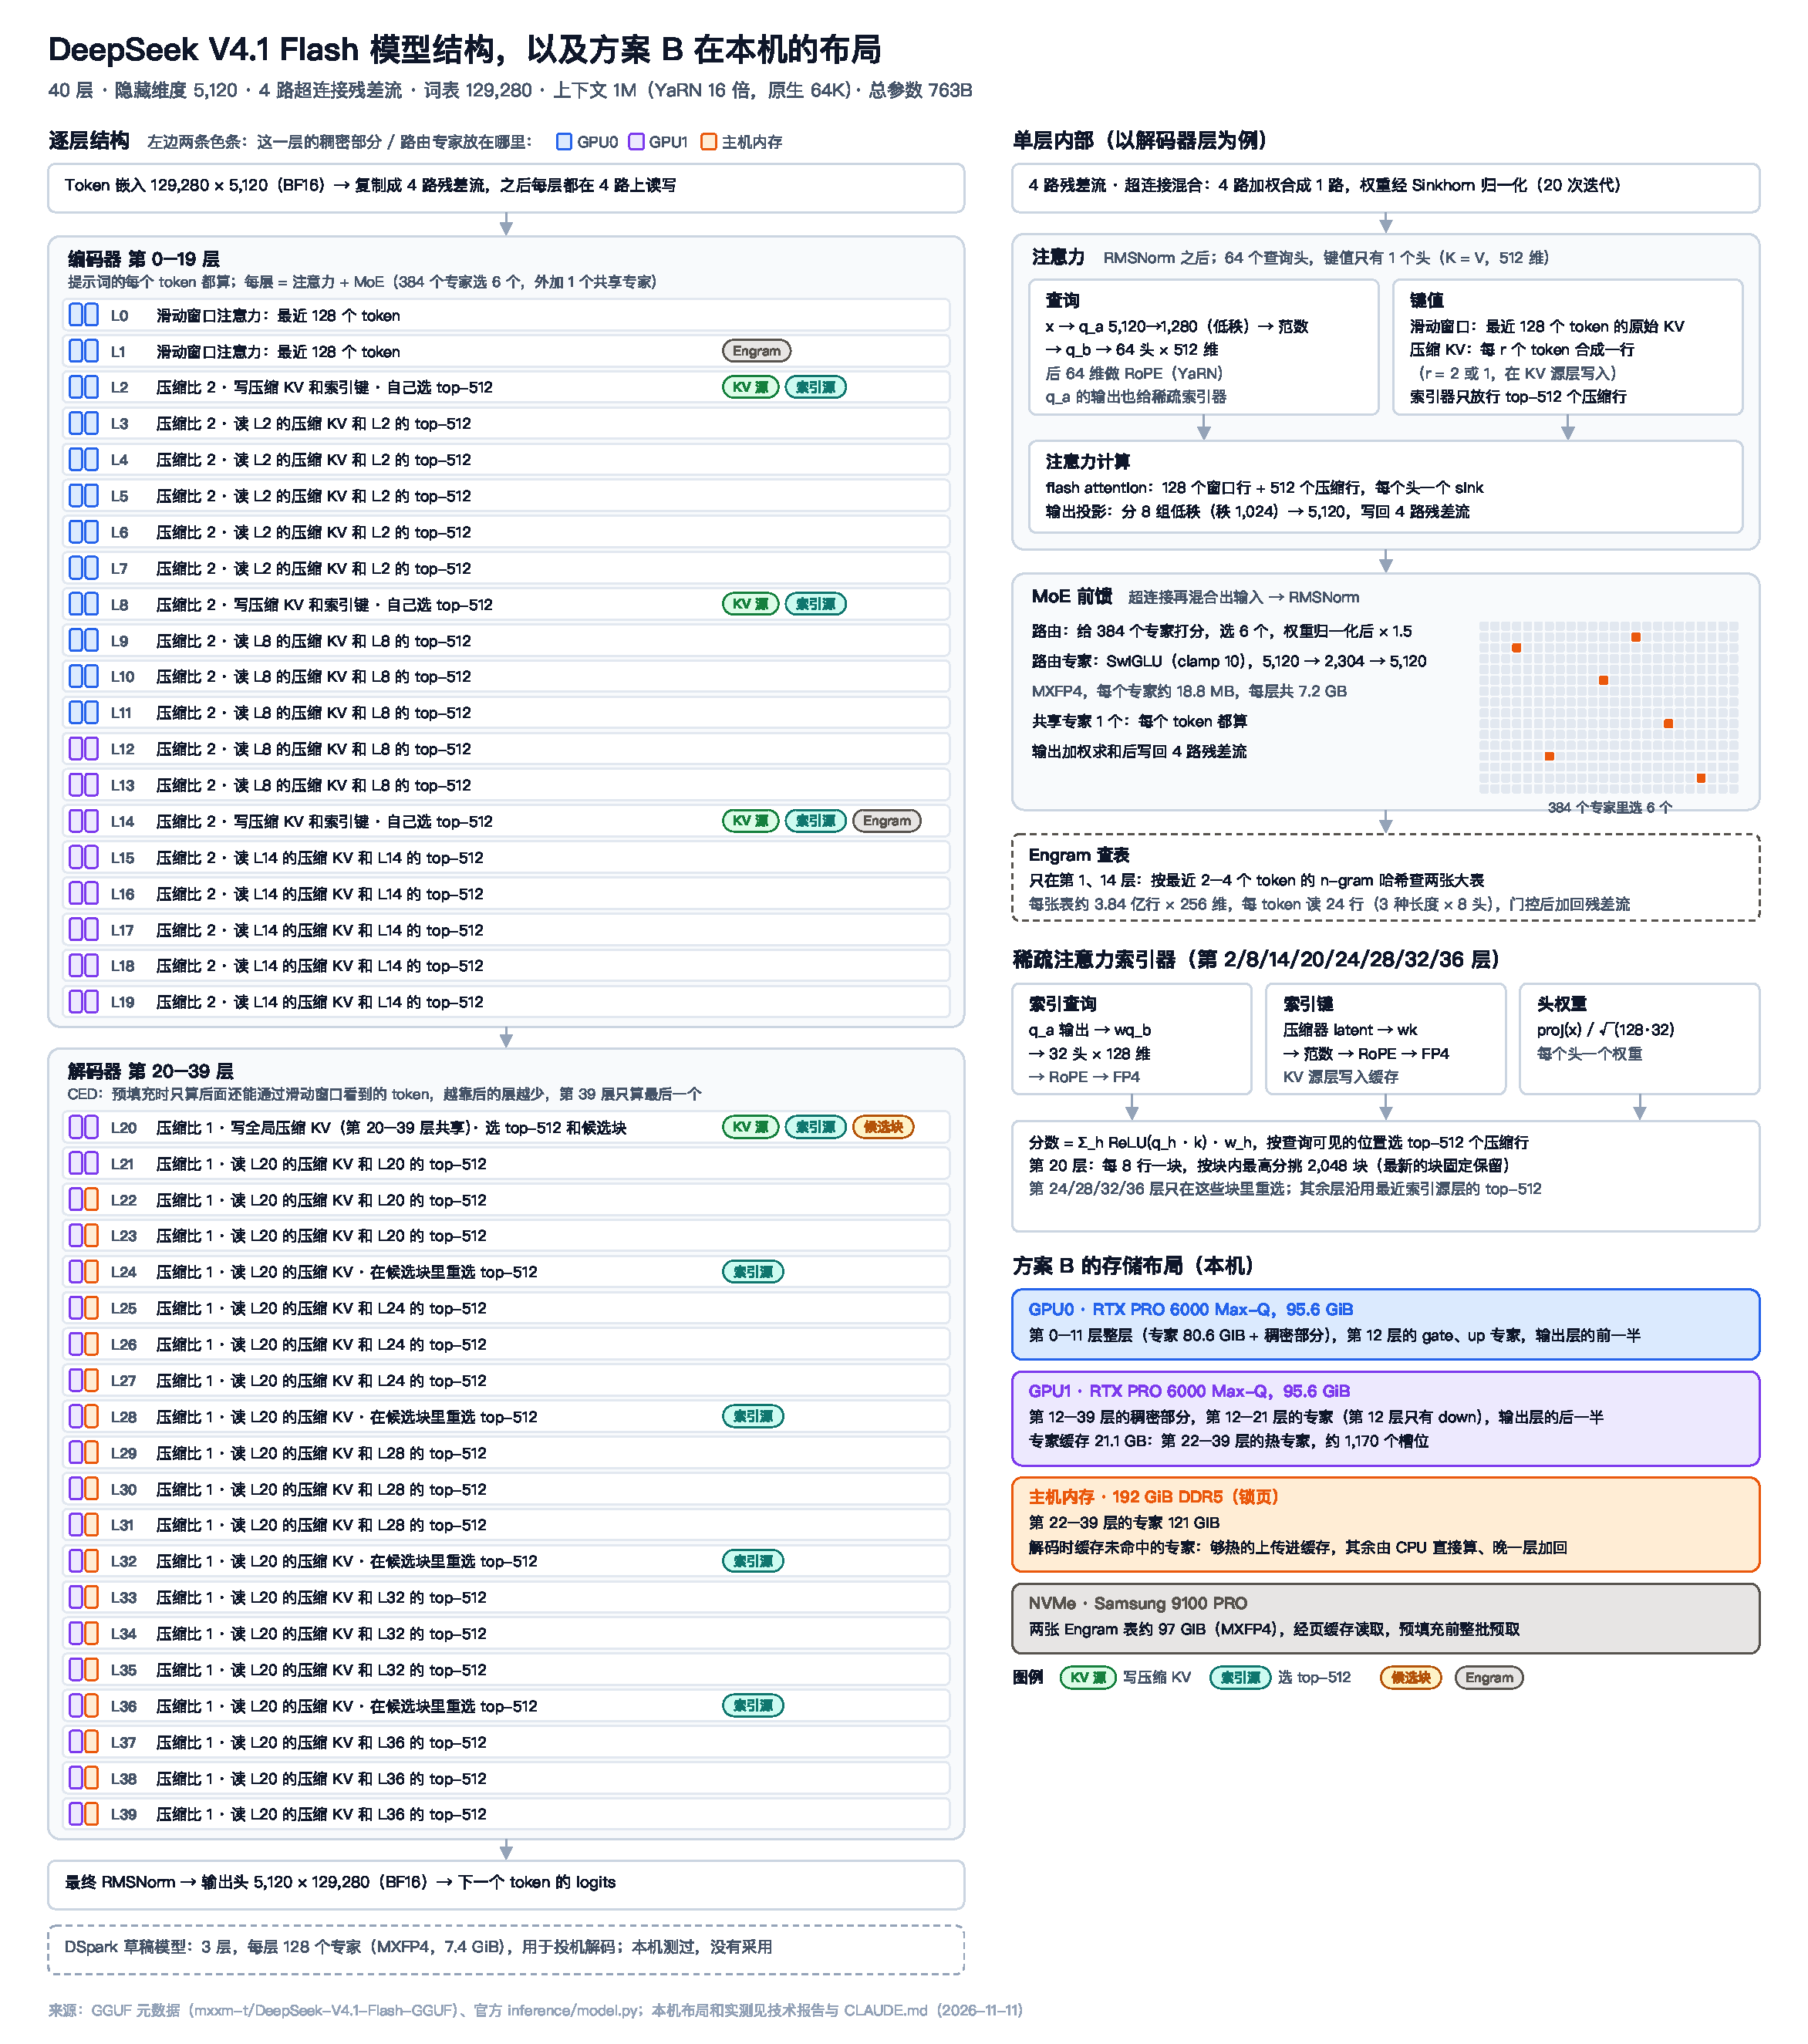
\includegraphics[width=18cm]{figures/architecture.pdf}}
  \caption{DeepSeek-V4.1-Flash 的逐层结构，以及方案 B 在本机的布局。左侧每行一层，色条表示该层稠密部分和路由专家所在的位置；右侧是单层内部、稀疏索引器和存储布局。}
  \label{fig:arch}
\end{figure}

\subsection{权重格式与量化}
\label{sec:formats}

本报告的优化都没有对模型再做量化：改动的只是权重放在哪一层，以及哪些 token、哪些行不必计算，每项改动都和改动前对拍（\S\ref{sec:floors}）。不过我们运行的 GGUF~\cite{mxllama} 本身和官方 checkpoint 不完全相同。表~\ref{tab:formats} 是逐个统计 12 个分片的结果。

\begin{table}[h]
  \centering
  \small
  \caption{GGUF 中各类权重的格式，与官方 checkpoint 对比。}
  \label{tab:formats}
  \begin{tabularx}{\textwidth}{@{}>{\raggedright\arraybackslash}p{3.2cm} >{\raggedright\arraybackslash}p{3.0cm} l r >{\raggedright\arraybackslash}X@{}}
    \toprule
    权重 & 官方 & GGUF & 大小 & 精度变化 \\
    \midrule
    路由专家 & FP4（E2M1，每 32 个一个缩放） & MXFP4 & 275.7 GiB & 无，同一种格式 \\
    注意力等稠密矩阵 & FP8 & Q8\_0 & 5.5 GiB & 很小，都是 8 bit，只是缩放方式不同 \\
    共享专家 & FP8\textsuperscript{*} & Q8\_0 & 1.5 GiB & 同上 \\
    \textbf{Engram 表} & \textbf{FP8，约 189 GiB} & \textbf{MXFP4} & \textbf{97.3 GiB} & \textbf{从 8 bit 降到 4 bit} \\
    嵌入、输出、路由门、压缩器、索引器投影 & — & BF16 & 2.8 GiB & 无 \\
    各种 norm、偏置 & — & F32 & 0.2 GiB & 无 \\
    \bottomrule
  \end{tabularx}
  \par\smallskip\raggedright\footnotesize *\ 按官方 \code{inference/model.py} 推断：只有路由专家用 FP4，其余线性层走 FP8 矩阵乘；共享专家没有单独核对。—：未单独核对，GGUF 中是 16 位或 32 位浮点。
\end{table}

真正降了精度的只有 Engram 表。转换 GGUF 时它从 FP8 压到了 MXFP4，体积减半，也更容易留在页缓存里。这是转换者的选择，我们直接继承；本报告的对拍都是同一个 GGUF 改动前后的比较，这一步对质量的影响没有测过，要测需要用官方 FP8 的表做参照。

计算时还有两处量化。GPU 和 CPU 上的矩阵乘都先把激活按 32 个一组量化成 int8 再乘，即 W4A8；官方参考实现用 FP8 激活，同为 8 bit。fork 在 Blackwell 上的预填充默认是 W4A4（激活只有 4 bit），我们改回了 8 bit（\S\ref{sec:floors}）。稀疏索引器的查询和键用 FP4，这是官方的设计，我们照官方实现做。KV cache 用默认的 F16，没有量化。

作为对比，方案 A 要把路由专家从约 4.25 bpw 再压到 3.0 bpw，相对原版的 KL 散度为 0.0545~\cite{diffbot}；方案 B 不做这一步，这正是选它的原因。

\subsection{方案 B 的布局}

方案 B 用层切分（\code{-sm layer -ts 12/29}）：GPU0 放第 0--11 层整层；GPU1 放第 12--39 层的稠密部分和第 12--21 层的专家；第 22--39 层的专家（121 GiB）放在锁页主机内存；Engram 表留在 NVMe，经页缓存读取。编码器的专家全部在显存，所以只要提示词不走解码器层，预填充就基本不碰主机内存。表~\ref{tab:place} 列出各层的内容。后来加入的 GPU1 专家缓存占 14 GB，大批次分流让 GPU0 的计算缓冲区多占约 1.9 GB；12.8 万上下文时，两张卡分别只剩约 3.6 GB 和 1.2 GB。

\begin{table}[h]
  \centering
  \small
  \caption{方案 B 的存储布局（最终配置）。}
  \label{tab:place}
  \begin{tabularx}{\textwidth}{@{}l X r@{}}
    \toprule
    位置 & 内容 & 容量 \\
    \midrule
    GPU0 & 第 0--11 层整层（专家 80.6 GiB + 稠密部分） & 95.6 GiB \\
    GPU1 & 第 12--39 层稠密部分，第 12--21 层专家 67.2 GiB，专家缓存 14 GB & 95.6 GiB \\
    主机内存 & 第 22--39 层专家 121 GiB（CUDA\_Host 锁页） & 192 GB \\
    NVMe & 两张 Engram 表（MXFP4，约 97 GiB） & 4 TB \\
    \bottomrule
  \end{tabularx}
\end{table}

% ---------------------------------------------------------------- 3
\section{评估方法}

\subsection{数值底线}
\label{sec:floors}

我们用 llama.cpp 的 KL 散度对拍：先存一份基准 logits，再比较改动后的 logits。早期的编译同一配置重跑完全相同（KLD 为 0）；加了后来的补丁后，重跑之间 KLD 平均约 0、最大约 6e-5，top-1 一致率 100\%。重要的发现是数值底线分两档（表~\ref{tab:floors}）：

\begin{itemize}
  \item 改动只落在解码器层（第 20--39 层）时，KLD 约 0.0005。例如把第 22--39 层的专家从 CPU 改到 GPU 上计算。
  \item 改动经过编码器层（第 0--19 层）时，0.005--0.01 属正常。例如只把第 5 层的专家改到 CPU 计算就是 0.0064；换内核、关融合、换 ubatch 也在这个量级。
\end{itemize}

原因在 CED：编码器的输出决定了所有位置共享的全局 KV，那里的舍入差别会扩散到之后所有位置；解码器层的差别只影响当前 token。判断一项改动是否正确，必须先确定它落在哪一档。

同一套方法一开始就查出了一个精度问题：mx-llama.cpp 在 Blackwell 上对 MXFP4 的预填充默认用 W4A4（激活量化到 4 bit），而官方参考实现是 W4A8。预填充路径对解码路径的 KLD 因此高达 0.044、top-1 一致率 91\%；改为 8 bit 激活后降到 0.012、95\%，与数值底线相当，预填充只慢约 5\%。

\begin{table}[h]
  \centering
  \small
  \caption{数值底线与 W4A4 问题（2026-10-21）。}
  \label{tab:floors}
  \begin{tabular}{@{}l l r@{}}
    \toprule
    比较 & 改动范围 & KLD \\
    \midrule
    同一配置重跑 & — & 0（后来最大 6e-5） \\
    第 22--39 层专家从 CPU 改到 GPU & 只有解码器层 & 0.0005 \\
    第 5 层专家从 GPU 改到 CPU & 经过编码器层 & 0.0064 \\
    预填充 W4A4 对解码路径 & 全部层 & 0.044 \\
    预填充 W4A8 对解码路径 & 全部层 & 0.012 \\
    \bottomrule
  \end{tabular}
\end{table}

\subsection{对官方实现的对拍}

KLD 只能说明最终输出变了多少，不能说明是哪一步造成的。对实现复杂的部分，我们写了独立的参照实现（oracle）逐层对拍：用 \code{llama-abyss-dump} 导出 fork 计算图里指定的张量，再用 PyTorch 按官方 \code{inference/model.py} 从同样的输入重算。解码步的注意力还用 float64 重算，单独量出内核的舍入误差。具体结果见 \S\ref{sec:indexer} 和 \S\ref{sec:gather}。

\subsection{剖析}

性能问题一律先剖析再动手。我们用 nsys 抓取一段预填充或一段解码，按设备统计内核、拷贝和空闲时间，再按 token 平均（\code{tools/eval/nsys\_breakdown.py}、\code{nsys\_decode.py}）。多轮智能体用一个模拟 Codex 的脚本测量：首轮带 4.8 万 token 的文档和两个工具，之后每轮回填约 1,500 token 的工具结果或追问，逐轮记录缓存复用和预填充时间（\code{agent-turns.sh}）。

% ---------------------------------------------------------------- 4
\section{解码}

方案 B 的原版解码是 16.5 \tps{}（空上下文），4 万上下文时约 14.6 \tps{}。瓶颈是 CPU：解码器后 18 层每个 token 要读 108 个专家、约 2.0 GB，而内存带宽只有 44 GB/s。

\subsection{GPU 专家缓存}

mx-llama.cpp 自带一个实验性的专家缓存：在 GPU1 上划出一组槽位（bank），每层一张「专家号 $\to$ 槽位号」的映射，命中的专家直接在 GPU 上算，未命中的同步上传并按 LRU 淘汰。我们给它 14 GB（约 780 个槽位，占第 22--39 层专家的 11\%）。真实文本的专家局部性很强，LRU 命中率约 75\%；4.8 万上下文的解码从 14.1 提升到 25.2 \tps{}，短上下文约 29--30 \tps{}，KLD 0.0005。

开启缓存后，我们在 PCIe Gen5 下剖析了 4.8 万上下文的解码（图~\ref{fig:decode}）：每 token 40.1 ms，其中 GPU1 上传未命中专家 17.4 ms（约 26.5 个、474 MiB），GPU1 内核 13.3 ms，GPU0 内核 4.8 ms，两卡都空闲 4.5 ms，几部分基本串行。上传是最大的一块。

\begin{figure}[t]
  \centering
  \begin{tikzpicture}
    \begin{axis}[abyss,
      xbar stacked, bar width=13pt,
      width=0.78\textwidth, height=4.6cm,
      xmin=0, xmax=62,
      xlabel={每 token 时间（ms）},
      ytick={1,2,3},
      yticklabels={{全部优化后，多轮会话}, {专家缓存，Gen5}, {专家缓存，GPU1 只有 Gen4}},
      y dir=reverse,
      ymajorgrids=false, xmajorgrids,
      legend columns=4, legend style={at={(0.5,1.04)},anchor=south,/tikz/every even column/.append style={column sep=8pt}},
      enlarge y limits=0.3]
      \addplot[fill=dsblue,draw=dsblue] coordinates {(14.7,1) (17.4,2) (33.3,3)};
      \addplot[fill=dsviolet,draw=dsviolet] coordinates {(10.4,1) (13.3,2) (13.3,3)};
      \addplot[fill=dslight,draw=dsblue] coordinates {(4.2,1) (4.8,2) (5.0,3)};
      \addplot[fill=dsgray,draw=dsgray] coordinates {(8.1,1) (4.5,2) (6.3,3)};
      \legend{上传专家, GPU1 内核, GPU0 内核, 两卡空闲}
    \end{axis}
  \end{tikzpicture}
  \caption{4.8 万上下文解码的每 token 时间（nsys，内存 3600 MT/s）。中间一行是只开专家缓存时；下面一行是一次开机后 GPU1 的链路只训练到 Gen4 时，上传慢了一倍（\S\ref{sec:incidents}）；上面一行是全部优化后、只追加的多轮会话中，每 token 37.5 ms（\S\ref{sec:realdecode}）。}
  \label{fig:decode}
\end{figure}

\subsection{解码注意力只取 top-k 行}
\label{sec:gather}

剖析还显示 GPU1 内核里有约 3 ms 花在 \code{concat\_cont} 上，而且随上下文增长：每层每个 token 都把滑动窗口和整个压缩 KV 拼成一个张量（4.8 万上下文时每次约 40 µs），再由 flash attention 按 top-512 掩码挑行。单个查询时这是浪费的：它只会看到 512 个压缩行。我们改为先用 \code{get\_rows} 取出这 512 行和它们的掩码，再和滑动窗口拼接，补齐到 256 的倍数后走普通 flash attention。

4.8 万上下文的解码从 27.7 提升到 30.6 \tps{}，12.8 万上下文从 23.9 提升到 30.9 \tps{}（都是同一提示词第二次生成，\S\ref{sec:realdecode}），解码速度基本不再随上下文变长而下降。server 上 temperature 0 生成的 top-20 KL 约 0.003，高于解码器层那一档底线。我们用 float64 对拍确认了原因：给定相同输入时，两条路径看到的是同一组 640 行，和 float64 的误差都约 5e-4（F16 舍入）；第 20 层的差别来自上游——第 2--19 层约 5e-4 的舍入差别经 MoE 在分数接近的专家之间选择而被放大，这正是「经过编码器层」那一档的机制。

\subsection{按热度准入的未命中分流}

原设计是把未命中全部交给 CPU 计算，只按静态热表换入。剖析后发现这行不通：LRU 的高命中率靠的是每个未命中都换入，不换入时命中率会掉到静态热表的水平（每 token 约 47 次未命中），CPU 计算反而比上传还慢；CPU 算完再把同一个专家上传，又要从内存读两遍。

我们改为按热度准入。每层由一个 CPU 算子规划：命中的照常读缓存；未命中的按衰减热度（每层每步乘 0.99）挑出一定比例，立即异步上传进 LRU 槽位；其余由 CPU 用主机内存里的原始专家计算，GPU 那边读 bank 末尾的全零槽位，down 之后两边相加。计算图里 CPU 分支先于 GPU 分支展开，规划算子在 CPU split 开头发出上传，CPU 计算其余未命中时 DMA 正在进行，每个专家只从内存读一遍。

表~\ref{tab:admit} 是上传比例的扫描。只上传一半，命中率不降：按热度挑出来的才进缓存，冷门专家不会把缓存冲掉。最终取 0.5：4.8 万上下文 36.1 \tps{}，12.8 万上下文 36.2 \tps{}，KL 约 2e-4，低于解码器层底线。这两个数和表里的速度一样，都是同一提示词第二次生成测出的，偏高；实际会话见下节。

\begin{table}[h]
  \centering
  \small
  \caption{未命中上传比例的扫描（4.8 万上下文，已开启 top-k 收集，复用提示词缓存后生成 256 token，即同一提示词第二次、一字不差的生成）。}
  \label{tab:admit}
  \begin{tabular}{@{}l r r r@{}}
    \toprule
    上传比例 & 解码（\tps） & 命中率 & 对全部上传的 top-20 KL \\
    \midrule
    全部上传（原缓存） & 30.6 & 75.5\% & — \\
    1.0（新路径） & 30.2 & 75.5\% & 0（逐位一致） \\
    0.5 & 36.1 & 75.9\% & 2.7e-4 \\
    0.4 & 35.7 & 75.1\% & 2.2e-4 \\
    0.3 & 36.4 & 74.5\% & 1.7e-4 \\
    0.2 & 36.0 & 73.1\% & 2.2e-4 \\
    0（全部交给 CPU） & 16.1 & 0\% & 1.8e-4 \\
    \bottomrule
  \end{tabular}
\end{table}

\subsection{实际会话中的解码速度}
\label{sec:realdecode}

Codex 的实际会话（上下文约 10 万 token）解码只有 30--31 \tps{}，明显低于表~\ref{tab:admit} 的 36。差别在测法：表里的速度来自同一提示词的第二次生成，temperature 0 下它和第一次一字不差，第一次用过的专家正好还在 LRU 缓存里，命中率偏高；同一脚本里第一次生成只有 32--35 \tps{}。Codex 自带的测速在短上下文下得到 47--49 \tps{}，也是同一段生成重复跑出来的。

我们改用只追加的会话测量（\code{decode\_modes.sh}）：首轮放文档和工具定义，之后每轮追加上一轮的回答和一个新问题，生成 256 个 token，轮换贪心或默认采样、流式或不流式。9.6 万上下文 27--31 \tps{}，4.8 万上下文 27--29 \tps{}，四种方式没有差别，和 Codex 的实际会话一致。所以解码既不受流式和采样影响，也不随上下文变长而变慢。

\begin{table}[h]
  \centering
  \small
  \caption{只追加的多轮会话中每 token 的时间（nsys，内存 3600 MT/s）。}
  \label{tab:realdecode}
  \begin{tabular}{@{}l r r@{}}
    \toprule
    部分 & 9.6 万上下文 & 4.8 万上下文 \\
    \midrule
    GPU1 上传未命中专家（约 20 个、360 MiB） & 14.5 ms & 14.7 ms \\
    GPU1 内核 & 10.5 ms & 10.4 ms \\
    GPU0 内核 & 4.2 ms & 4.2 ms \\
    两卡都空闲 & 7.9 ms & 8.1 ms \\
    合计（nsys 下） & 37.1 ms & 37.5 ms \\
    \bottomrule
  \end{tabular}
\end{table}

表~\ref{tab:realdecode} 是剖析结果。和上下文长度有关的内核（注意力、索引器打分、top-k、取行和拼接）在 9.6 万上下文时合计只有约 2 ms，top-k 已经是基数选择。一个解码器层的时间线是：GPU1 先算上一层专家的合并、本层注意力和路由（127 个内核，约 0.47 ms）；路由结果和本层输入传回主机后，上传 1 个未命中的专家（3 × 6.3 MB，约 0.70 ms），同时 CPU 算另一个（约 0.79 ms）；之后 CPU 结果传回、启动下一段计算图（约 0.09 ms）。上传和 CPU 计算同时从内存读约 37.6 MB，用了约 0.8 ms，已经到内存带宽的上限；而 GPU 上能挪到上传期间去算的只有本层命中的专家，每层不到 0.1 ms。所以解码剩下的时间主要是每层串行的未命中处理，把上传和命中专家的计算并行起来，每 token 最多省 2--3 ms。

% ---------------------------------------------------------------- 5
\section{预填充}

原版对提示词也跑完 40 层：每个 2,048 token 的 ubatch 都要把主机内存里 121 GiB 的解码器专家读一遍。4.8 万 token 的提示词因此要 135 s（约 355 \tps{}）。

\subsection{CED 感知预填充}

官方参考实现对提示词也跑满 40 层，CED 体现在 KV 的共享方式上：解码器层只有滑动窗口用到各层自己的隐状态。因此可以精确地裁剪：第 0--19 层全部 token 都算；第 39 层只算最后一个 token；第 $L$ 层（20--38）只需算最后 $128 + 127 \times (38-L)$ 个 token——每往前一层，滑动窗口让依赖往前延伸 127 个 token。实现原本在末尾多留 256 个位置，给投机解码的回退用；没开 DSpark 时 DSV4 不能部分回退，后来改为默认不留（\S\ref{sec:tailmerge}）。这样解码器层合计约 2.4 万个「token × 层」，与提示词长度无关；4.8 万 token 的提示词在原版中是 $20 \times 48{,}240 \approx 96$ 万个（图~\ref{fig:ced}）。

\begin{figure}[t]
  \centering
  \begin{tikzpicture}
    \begin{axis}[abyss,
      width=0.92\textwidth, height=5.0cm,
      ymode=log, ymin=0.6, ymax=1e5,
      xmin=-1, xmax=40,
      xlabel={层}, ylabel={计算 FFN 的 token 数},
      xtick={0,5,10,15,20,25,30,35,39},
      legend style={at={(0.02,0.08)},anchor=south west}]
      \addplot[dsgray, mark=none, line width=1pt, dashed] coordinates {(0,48240) (39,48240)};
      \addplot[dsblue, mark=*, mark size=1.2pt, line width=1pt] coordinates {
        (0,48240) (1,48240) (2,48240) (3,48240) (4,48240) (5,48240) (6,48240) (7,48240) (8,48240) (9,48240)
        (10,48240) (11,48240) (12,48240) (13,48240) (14,48240) (15,48240) (16,48240) (17,48240) (18,48240) (19,48240)
        (20,2414) (21,2287) (22,2160) (23,2033) (24,1906) (25,1779) (26,1652) (27,1525) (28,1398) (29,1271)
        (30,1144) (31,1017) (32,890) (33,763) (34,636) (35,509) (36,382) (37,255) (38,128) (39,1)};
      \legend{原版, CED 感知预填充}
    \end{axis}
  \end{tikzpicture}
  \caption{4.8 万 token 提示词每层计算 FFN 的 token 数（按实现中的规划规则计算，没开 DSpark 时不留余量）。编码器层全部计算；解码器层只计算后面还能通过滑动窗口看到的 token。}
  \label{fig:ced}
\end{figure}

实现分两步。第一步（\code{0003}）只跳过 FFN，注意力仍对所有 token 计算，KV 写入完全不变；被跳过的 token 之后各层的隐状态不正确，但只会进入没有后续 token 读取的滑动窗口。每次 \code{llama\_decode} 按自己的末尾规划，所以 server 用 \code{-b 65536} 让整段提示词进一次调用。4.8 万 token 的预填充从 135 s 降到 41.8 s，8k/16k 上下文对拍 KLD 0.00006 / 0.00004，top-1 一致率 99.8\%。

第二步（\code{0005}）先剖析：此时 41.8 s 里第 20--39 层的注意力占 19.9 s。我们让这些层仍为所有 token 写 KV，但只对 CED 子集取出查询和掩码行计算注意力。预填充降到 27.9 s（1,715 \tps{}），KLD 0.00004--0.00007，temperature 0 的输出和第一步一字不差。

\subsection{Engram 预取}

Engram 表以 mmap 映射且设了随机访问提示，每次缺页都同步读一个 4 KiB 页，2,048 个 token 约需 2.4 s，瓶颈在缺页延迟而不在 SSD 带宽。由于行号只取决于输入 token，我们在 \code{llama\_decode} 拿到整批后立即算出全部行号，由 8 个后台线程按地址排序后用 \code{MADV\_WILLNEED} 预读。页缓存冷时，4.8 万 token 的预填充从 91.1 s 降到 54.3 s，冷读开销从约 39 s 降到约 2 s；热缓存时不变，结果与不预取完全一致。冷读已基本藏在计算后面，io\_uring 和按行缓存等后续步骤暂缓。

\subsection{补上官方稀疏索引器}
\label{sec:indexer}

fork 原本对 V4.1 的压缩 KV 做稠密注意力。压缩行在 512 以内时与官方的 top-512 选择等价，更长时就不同了：压缩比 1 的层超过约 512 个 token、压缩比 2 的层超过约 1,024 个 token 之后。智能体的上下文几乎都在这个范围里，所以这首先是正确性问题。

我们按官方 \code{inference/model.py} 补上了完整的索引器：KV 源层写 FP4 索引键（每 32 个一块，缩放 $2^{\lceil \log_2(\mathrm{amax}/6) \rceil}$），索引源层计算 $\sum_h \mathrm{ReLU}(q_h \cdot k)\, w_h$ 并选 top-512，第 20 层挑候选块，其余层沿用最近索引源的结果；flash attention 只看选中的位置。512 token 以内与稠密版 KLD 为 0；8k/16k/32k 上下文时，稀疏版的 PPL 比稠密版低 0.9\% / 3.1\% / 0.23\%（表~\ref{tab:sparse}）。由于注意力只看 640 行，4.8 万 token 的预填充也从 27.9 s 降到 22.7 s，12.8 万 token 为 51.8 s（2,464 \tps{}）。

\begin{table}[h]
  \centering
  \small
  \caption{稀疏索引器对稠密注意力（perplexity，每档 4 段）。}
  \label{tab:sparse}
  \begin{tabular}{@{}l r r r r@{}}
    \toprule
    上下文 & PPL（稠密） & PPL（稀疏） & 变化 & 稀疏对稠密 KLD \\
    \midrule
    8k & 6.023 & 5.972 & $-0.9\%$ & 0.057 \\
    16k & 3.009 & 2.916 & $-3.1\%$ & 0.094 \\
    32k & 1.0027 & 1.0004 & $-0.23\%$ & 0.012 \\
    \bottomrule
  \end{tabular}
\end{table}

为确认实现与官方一致，我们导出第 2、20、24 层的索引器输入输出，用三种算术重算 top-512 并比较重合率（表~\ref{tab:oracle}）：全程 float32；fork 的算术（Q8\_0 矩阵乘把激活量化成 int8）；官方的算术（bf16 激活，量化成 e4m3 后做 FP8 GEMM）。fork 与自己的算术重合 99.98\% 以上，说明 RoPE/YaRN、FP4、权重缩放、可见性和 top-k 每一步都对；fork 离 float32 的距离（98.7--99.2\%）比官方算法自己离 float32 的距离（97.1--98.7\%）还近。索引键 99.99\% 以上逐位一致，不一致的都是恰好落在 FP4 中点上的单个元素。

\begin{table}[h]
  \centering
  \small
  \caption{top-512 集合的平均重合率（4,027 token 提示词）。}
  \label{tab:oracle}
  \begin{tabular}{@{}l r r r r@{}}
    \toprule
    层 & fork 对 int8 参照 & fork 对 float32 & 官方算术对 float32 & fork 对官方算术 \\
    \midrule
    2 & 99.99\% & 99.16\% & 98.67\% & 98.63\% \\
    20 & 99.98\% & 98.67\% & 97.14\% & 97.11\% \\
    24 & 99.98\% & 98.85\% & 97.40\% & 97.36\% \\
    \bottomrule
  \end{tabular}
\end{table}

\subsection{大批次分流}

多轮会话里每轮新增的 token 不多，但只要批次超过 32 个 token，第 22--39 层几乎全部 384 个专家都会被用到，调度器把这些大批次的专家矩阵乘卸载到 GPU0，每层整批上传。一轮 1,610 token 的预填充（7.0 s）中，GPU0 上传 145 GiB 用了 5.4 s，而 CPU、GPU1 的链路和专家缓存都闲着。这部分的下限是把这些专家从内存读一遍，约 3 s。

我们把未命中分流的思路推广到大批次：每层一个 CPU 算子统计每个专家的 token 数，按从少到多把专家交给 CPU，直到 CPU 的预计时间追上其余专家的上传时间；其余照常上传到 GPU0。为此给 CUDA 的 MMQ 补上了 id = $-1$ 的处理（跳过并把输出清零），上传回调直接用规划算子在主机上的结果，不必从 GPU 读回 id。

第一版的 CPU 分支处理整块张量（全部 token × 6 个专家），而 CPU 实际只算约 5\% 的行，量化、SwiGLU、清零和 252 MB 输出的回传把收益全吃掉了，比不分流还慢。改为紧凑批次后——只取出交给 CPU 的「token × 专家」（最多 1,024 行），在 GPU1 上取出这些 token，CPU 上按一行一个专家计算，\code{set\_rows} 写回后与 GPU0 的结果相加——2,048 token 一批的预填充从 4.88 s 降到 4.24 s，KLD 0.00046。多轮会话之后每轮的预填充从 5.7--7.2 s 降到 4.6--5.6 s，首轮从 30.6 s 降到 27.9 s（图~\ref{fig:agent}）。

\begin{figure}[t]
  \centering
  \begin{tikzpicture}
    \begin{axis}[abyss,
      width=0.92\textwidth, height=5.0cm,
      ybar, bar width=10pt, ymin=0, ymax=8.5,
      xlabel={轮次（每轮新增 1,200--1,600 token）}, ylabel={预填充时间（s）},
      xtick={2,3,4,5,6},
      nodes near coords={\pgfmathprintnumber[fixed,fixed zerofill,precision=1]{\pgfplotspointmeta}},
      nodes near coords style={font=\scriptsize},
      legend columns=3, legend style={at={(0.5,1.03)},anchor=south,/tikz/every even column/.append style={column sep=10pt}},
      enlarge x limits=0.15]
      \addplot[fill=dslight,draw=dsblue] coordinates {(2,5.8) (3,6.1) (4,5.7) (5,7.0) (6,7.2)};
      \addplot[fill=dsblue,draw=dsblue] coordinates {(2,4.7) (3,4.9) (4,4.6) (5,5.6) (6,5.6)};
      \addplot[fill=dsviolet,draw=dsviolet] coordinates {(2,3.3) (3,3.2) (4,3.0) (5,2.9) (6,3.5)};
      \legend{不分流, 大批次分流, 末段一遍算完}
    \end{axis}
  \end{tikzpicture}
  \caption{多轮智能体会话中每轮的预填充时间（首轮为 4.8 万 token 的文档，之后每轮回填工具结果或追问；内存 3600 MT/s）。末段一遍算完见 \S\ref{sec:tailmerge}。}
  \label{fig:agent}
\end{figure}

这一步离下限还有约 30 ms/层：GPU0 的上传暂存区在 gate、up、down 三份权重之间复用，每段之间都要同步，CPU 要等 gate 那批传完才能开始；CPU 计算和 DMA 又共享 44 GB/s 的内存带宽。合并的几步要固定在 GPU0，否则 GPU1 的计算缓冲区会大 3.7 GB，12.8 万上下文时放不下。实现中还发现并修复了 fork 的一处问题（\code{0013}）：\code{ggml\_backend\_sched\_reserve\_size} 在切分计算图之前重置调度器，清掉了构建计算图时手动指定的后端，按错误的切分估算计算缓冲区。

\subsection{末段一遍算完}
\label{sec:tailmerge}

CED 让每次 \code{llama\_decode} 调用都按自己的末尾跑解码器层，凡是超过 32 个 token 的调用都要把第 22--39 层几乎全部专家从内存读一遍。server 为了建检查点，会在最后一条用户消息开头、末尾前 4 + n\_ubatch 和末尾前 4 处拆调用。生产日志里 Codex 的大多数轮次因此被拆成两次大调用（例如 1,772 + 866 + 4），比同样长度只有一次调用的轮次多花 1.5--2 s；一次调用里末段跨两个 ubatch 时，也要读两遍。我们做了三处改动（\code{0015}）：

\begin{itemize}
  \item 提示词最后 2,700 个 token 里不再按用户消息开头和末尾前 4 + n\_ubatch 拆调用，只留末尾前 4 个 token 那次，下一轮靠它从助手前缀处接着算。会话的第一个检查点照旧，Codex 的辅助请求靠它复用系统提示。代价是这两类检查点没了：只有改写最后一条用户消息时才用得上，这时 server 退回上一轮的检查点，多算这一轮。
  \item 一次调用的余数放进第一个 ubatch，最后一个 ubatch 是满的 2,048 个。原来余数在最后，最后一个 ubatch 常常只有几百个 token，第 20--32 层左右都要在前一个 ubatch 里再算一遍；现在前一个 ubatch 只剩第 20--22 层的少量 token。
  \item 末尾的余量默认等于回退环的深度 \code{n\_rs\_seq}，没开 DSpark 时为 0。我们按规划公式逐个位置核对过，余量为 0 时下一个 token 需要的滑动窗口状态仍然完整。
\end{itemize}

\begin{table}[h]
  \centering
  \small
  \caption{末段一遍算完的效果（\code{agent-turns.sh}，内存 3600 MT/s）。}
  \label{tab:tailmerge}
  \begin{tabular}{@{}l r r@{}}
    \toprule
    配置 & 首轮 4.8 万 token & 之后 5 轮（1,200--1,600 token） \\
    \midrule
    改动前 & 27.9 s & 4.6--5.6 s \\
    末段不拆调用 & 25.3 s & 3.2--3.7 s \\
    + 最后一个 ubatch 对齐到满 & 24.4 s & 3.2--3.7 s \\
    + 余量为 0 & 24.0 s & 2.9--3.5 s \\
    \bottomrule
  \end{tabular}
\end{table}

新提示词按外部测速的方式（关闭 prompt 缓存，每档 3 次取中位数）测，2,324 token 从 5.57 s 降到 3.69 s，4,277 token 从 8.80 s 降到 4.34 s。对拍方面，最后一个 ubatch 对齐对改动前的 KLD 是 0.0092、top-1 一致率 95.4\%，和只把 ubatch 从 2048 改成 1024 的 0.0090、96.0\% 一样；余量 0 对余量 256 生成的 256 个 token 全部相同（top-20 KL 4.6e-4）。我们还用 token 数组直接构造提示词，让调用长度除以 2,048 余 0、1、2、7--9、31--33、127--129、1000、2047，各测约 2 千、4 千、2 万 token，42 个请求全部正常。

% ---------------------------------------------------------------- 6
\section{服务与智能体负载}

\subsection{多轮会话的缓存复用}

V4.1 的缓存不能回退到滑动窗口中间，只能退回检查点。server 在每条用户消息的开头、最后一条用户消息开头和提示词末尾附近创建检查点。模拟会话中，从第 3 轮起每轮只重算上一轮生成的回复加 4 个 token：回复经模板重新渲染后与生成时的 token 不完全一样，server 退回到「Assistant」前缀处的检查点。

\subsection{prompt 缓存的选择}

在 Codex 的 6 个真实请求中（预填充合计 76 s，生成 129 s），我们发现 server 只有一个槽位，Codex 的辅助请求（与主对话共享约 4,500 token 的系统提示和工具定义，只问一句）会把主对话挤出槽位。server 已把主对话存进内存里的 prompt 缓存，但主对话回来时，槽位里的辅助请求与它仍有 94\% 的前缀相同，而 server 只在保留比例低于一半时才去缓存里找，并且按保留比例挑选，长的条目反而落选。

我们改为按「能直接用上的 token 数」比较槽位和缓存条目——对检查点受限的缓存，就是不晚于分叉点的最近检查点的位置——多出 256 个以上就换入；只用到一小部分的条目复制一份，原条目留在缓存里。另一个问题是辅助请求自己也从头算：系统提示末尾有检查点，但 server 要求检查点比分叉点早至少 128 个 token。这是为保存滑动窗口的检查点定的规则；V4.1 的检查点是那个位置的完整状态（\code{pos\_min == pos\_max}），在分叉点之前就能接着算。修复后，同一场景里辅助请求从 8.4 s 降到 0.3 s（只重算 13 个 token），主对话的下一轮从内存缓存换回，只重算 216 个 token、2.2 s。

\subsection{真实负载暴露的缺陷}
\label{sec:incidents}

\begin{itemize}
  \item \textbf{未分配的输入张量}。CED 让某些层在某个 ubatch 里没有 token，依赖它们的计算被整段丢掉，预先建好的输入张量就不会分配，往里写数据时断言失败。这在 CED 行映射（提示词约 2,500--16,000 token）和候选块输入（约 1.7 万 token 以上、长度除以 2,048 余约 114--622）上各出现一次，都只在特定长度下触发，测速用的 4.8 万和 12.8 万 token 恰好都没碰到，由 Codex 的请求暴露。
  \item \textbf{全零槽位重复}。未命中分流最初只有一个全零槽位。9--32 token 的批次里，同一 token 的多个 CPU 未命中指向同一个槽位，CUDA MMQ 的重排每个专家每个 token 只记一行，漏掉的行号未初始化，量化内核越界。改为每个 token 的第 $k$ 个专家用第 $k$ 个全零槽位。
  \item \textbf{PCIe 降速}。有一次开机后 GPU1 的链路只训练到 Gen4，主机到 GPU1 只有 14.4 GB/s，未命中上传慢了一倍，解码从约 25 掉到 17 \tps{}（图~\ref{fig:decode}）；重启后恢复。改 BIOS 后第一次开机又出现一次，GPU1 只到 Gen3，主机到 GPU1 只有 1.78 GB/s，同样重启恢复。测速脚本现在会先检查链路。
  \item \textbf{测试 server 退出时卡住}。测试 server 收到退出信号时正好接到外部请求，之后 GPU 和 CPU 都是 0\%，只能强制结束。生产 server 重启时也可能碰到。
  \item \textbf{Codex 的 MCP 工具被丢弃}。Codex 每个请求带的 9 个 \code{namespace} 类型工具，server 不支持，直接跳过，模型看不到。这个问题还没有修。
\end{itemize}

% ---------------------------------------------------------------- 7
\section{把内存提到 5200 MT/s}

4 × 48 GB 双 rank、每通道两条时，AMD 默认只跑 3600 MT/s。内存条标称 5600，SPD 里的 XMP 和 EXPO 配置都是 DDR5-6000、1.40 V。我们在 BIOS 里设 EXPO I，再把频率降到 DDR5-5200，并关掉 Memory Context Restore。stressapptest 用 150 GB 压 1 小时通过，没有硬件错误，内存条最高 62 °C；同一编译重跑的对拍和改之前一致，差别和这个编译两次运行之间一样。

\begin{table}[h]
  \centering
  \small
  \caption{内存从 3600 提到 5200 MT/s 前后（2026-10-25）。}
  \label{tab:ddr5200}
  \begin{tabular}{@{}l r r@{}}
    \toprule
    测试 & 3600 MT/s & 5200 MT/s \\
    \midrule
    内存纯读 & 44 GB/s & 54 GB/s \\
    两卡同时从主机读 & 43.4 GB/s & 50.6 GB/s \\
    单卡从主机读 & 28.9 GB/s & 28.9 GB/s \\
    9.6 万上下文多轮会话解码 & 29.0--31.1 \tps{} & 30.7--33.0 \tps{} \\
    多轮智能体首轮 / 之后每轮 & 24.0 / 2.9--3.5 s & 23.1 / 2.7--3.2 s \\
    新提示词 604 / 2,324 / 4,277 token & 2.59 / 3.69 / 4.34 s & 2.27 / 3.35 / 4.01 s \\
    \bottomrule
  \end{tabular}
\end{table}

各项快了 6--12\%，少于我们预计的 15--20\%。解码时上传到 GPU1 受 PCIe 限制，每个专家约 0.7 ms，和内存频率无关，只有 CPU 算的那一半变快了。内存带宽也只提高了 23\%，理论上是 44\%，可能是内存控制器频率被自动设成了内存频率的一半，还没有确认。专家缓存的上传比例（0.5）是在 3600 MT/s 下定的，现在 CPU 快了，可能不再最优。

% ---------------------------------------------------------------- 7
\section{结论、局限与未来方向}

在一台双卡工作站上，Abyss 以原生 MXFP4 精度运行 DeepSeek-V4.1-Flash：只追加的多轮会话里单流解码 31--33 \tps{}，4.8 万和 9.6 万上下文一样；4.8 万 token 提示词的预填充约 23 s，多轮会话每轮约 3 s。收益主要来自四类工作：顺着模型结构减少计算（CED 感知预填充、稀疏索引器、解码注意力只取 top-k），按热度安排数据所在的层级（专家缓存与准入），让 CPU、DMA 和 GPU 同时工作（未命中分流、大批次分流），以及减少重复读取（末段一遍算完）。每一项都先剖析、后实现，并用分档的数值底线和对官方实现的对拍确认正确性。

\paragraph{局限。} 解码器专家的读取最终受内存带宽和 PCIe 限制：每个未命中的专家都要从双通道内存读一遍，上传的那一半还要经过 x8 的 PCIe（每个约 0.7 ms），而且一层接一层串行；预填充的大批次也已接近「每层专家读一遍」的下限。GPU1 的链路两天里两次没有训练到 Gen5，每次开机后都要先检查。显存余量很小（12.8 万上下文时两卡分别约 3.6 GB 和 1.2 GB），更大的缓存或更长的上下文要以缩小专家缓存为代价。GGUF 中的 Engram 表从官方的 FP8 降到了 MXFP4（\S\ref{sec:formats}），这对质量的影响还没有测过。DSpark 投机解码在 V4.1 上尚不支持，这部分收益还没有拿到。

\paragraph{未来方向。}
\begin{itemize}
  \item 在 5200 MT/s 下重新扫专家缓存的上传比例，并确认内存控制器是否和内存同频。
  \item 合并 GPU 上的小内核：解码时每 token 约 2,900 个内核、14.6 ms，占四成多，平均每个只有约 5 µs。
  \item 让上传和本层命中专家的计算并行，并减少每层的同步，预计每 token 省 2--3 ms。
  \item 补上 V4.1 的 DSpark 投机解码。diffbot 在智能体编程会话中开启后解码约为单流的两倍；但在分层布局下，一次验证多个 token 会选中更多不同的专家，要多读的专家可能抵消一部分收益，需要实测。
  \item 与方案 A（3.0 bpw 专家、vLLM 双卡张量并行，预计 55--75 \tps{}）做一次同机对比，量化速度与精度的取舍。
\end{itemize}

\begin{thebibliography}{9}
\bibitem{v41} DeepSeek-AI. DeepSeek-V4.1-Flash: Pushing the Limits of KV Cache Compression. 2026. \url{https://huggingface.co/deepseek-ai/DeepSeek-V4.1-Flash}
\bibitem{mxllama} mxxm-t. mx-llama.cpp 与 DeepSeek-V4.1-Flash 的 MXFP4 GGUF. \url{https://huggingface.co/mxxm-t/DeepSeek-V4.1-Flash-GGUF}
\bibitem{diffbot} diffbot. DeepSeek-V4.1-Flash-EXL3-3bpw-2x-RTX-PRO-6000. \url{https://huggingface.co/diffbot/DeepSeek-V4.1-Flash-EXL3-3bpw-2x-RTX-PRO-6000}
\bibitem{strata} Strata：三层分工的本地 MoE 推理. \url{https://github.com/Niko1221/Strata}
\end{thebibliography}

\newpage
\appendix

\section{补丁清单}

Abyss 的全部改动以补丁形式保存在仓库的 \code{mx-llama.cpp/} 目录，基于 mx-llama.cpp 的提交 \code{c4d12e2}，按序号依次应用。

\begin{table}[h]
  \centering
  \small
  \begin{tabularx}{\textwidth}{@{}l X l@{}}
    \toprule
    补丁 & 作用 & 开关 \\
    \midrule
    0001 & server 的专家命中统计 & \code{ABYSS\_EXPERT\_STATS} \\
    0002 & V4.1 的工具调用标签（DSML，标签名带前导空格） & — \\
    0003 & CED 感知预填充：解码器层只算可见 token 的 FFN & \code{ABYSS\_CED\_PREFILL=1} \\
    0004 & Engram 整批预取 & \code{ABYSS\_ENGRAM\_PREFETCH=8} \\
    0005 & CED 感知预填充：注意力也只算子集 & 同 0003 \\
    0006 & V4.1 稀疏注意力索引器 & \code{ABYSS\_DSV41\_INDEXER=1} \\
    0007 & \code{llama-abyss-dump}：导出计算图张量用于对拍 & — \\
    0008 & 单 token 解码时注意力只取 top-k 行 & \code{ABYSS\_DSV41\_DECODE\_GATHER=1} \\
    0009 & 专家缓存未命中按热度分给上传和 CPU & \code{ABYSS\_MOE\_CPU\_MISS=1} \\
    0010 & 修 CED 行映射未分配；未命中分流的全零槽位重复 & — \\
    0011 & 修候选块输入未分配 & — \\
    0012 & prompt 缓存按能直接用上的 token 数挑选 & — \\
    0013 & 修调度器估算显存时清掉手动指定的后端 & — \\
    0014 & 预填充大批次分流到 CPU & \code{ABYSS\_MOE\_BIG\_SPLIT=1} \\
    0015 & 提示词末段一遍算完；CED 余量跟 \code{n\_rs\_seq} & \code{ABYSS\_CKPT\_TAIL\_MERGE=2700} \\
         & & \code{ABYSS\_CED\_ALIGN=1} \\
    \bottomrule
  \end{tabularx}
\end{table}

\section{复现}

生产配置的启动命令（需打过全部补丁的编译；还必须设 \code{GGML\_CUDA\_Q8\_1\_CACHE=0} 和 \code{GGML\_CUDA\_MMQ\_PREC=q8}；内存在 BIOS 里设 EXPO I + DDR5-5200）：

\begin{small}
\begin{verbatim}
GGML_CUDA_Q8_1_CACHE=0 GGML_CUDA_MMQ_PREC=q8 \
ABYSS_CED_PREFILL=1 ABYSS_ENGRAM_PREFETCH=8 ABYSS_DSV41_INDEXER=1 \
ABYSS_DSV41_DECODE_GATHER=1 ABYSS_MOE_CPU_MISS=1 ABYSS_MOE_BIG_SPLIT=1 \
ABYSS_CKPT_TAIL_MERGE=2700 ABYSS_CED_ALIGN=1 \
llama-server -m DeepSeek-V4.1-Flash-MXFP4-00001-of-00012.gguf \
  -ngl 99 -sm layer -ts 12/29 -fa 1 -lm dio -c 131072 -b 65536 -ub 2048 \
  -ot "blk\.(2[2-9]|3[0-9])\.ffn_(gate|up|down)_exps\.=CPU" \
  -t 16 -np 1 --moe-cache-mib 14000 \
  --jinja --chat-template-file deepseek-v4.1.jinja
\end{verbatim}
\end{small}

评估脚本在仓库的 \code{tools/eval/}，复制到机器上运行，运行前要先停 server：

\begin{center}
  \small
  \begin{tabular}{@{}l l@{}}
    \toprule
    脚本 & 用途 \\
    \midrule
    \code{kl.sh} & 存基准 logits，比较 KLD \\
    \code{bench.sh} & 解码与预填充测速 \\
    \code{prefill-warm.sh} & server 热缓存预填充 \\
    \code{profile-prefill.sh}、\code{profile-decode.sh} & nsys 剖析预填充、解码 \\
    \code{dump-indexer.sh}、\code{indexer\_oracle.py} & 稀疏索引器的单层对拍 \\
    \code{decode-gather.sh}、\code{decode\_attn\_oracle.py} & 解码注意力的 float64 对拍 \\
    \code{engram-cold.sh}、\code{engram-share.sh} & Engram 冷读开销与占比 \\
    \code{m2-cpu-miss.sh} & 未命中分流的上传比例扫描 \\
    \code{agent-turns.sh} & 多轮智能体会话 \\
    \code{decode\_modes.sh} & 只追加的长会话里测解码，\code{CAPTURE=1} 剖析 \\
    \code{prefill-sizes.sh} & 几种长度新提示词的预填充 \\
    \bottomrule
  \end{tabular}
\end{center}

\section{术语表}
\label{sec:glossary}

按主题分组；同一个词在不同语境下含义不同的（如「解码器层」和「解码」、server 的槽位和专家缓存的槽位），在条目里分别说明。

\setlist[description]{font=\normalfont\bfseries,leftmargin=0pt,itemsep=0.25em}

\subsection*{模型结构}
\begin{description}\small
  \item[MoE（混合专家）] 每层有许多个前馈网络（专家），每个 token 只由路由器挑出其中几个来算。V4.1-Flash 每层 384 个路由专家，每个 token 选 6 个，另有 1 个共享专家每个 token 都算。
  \item[路由器（gate）] 每层给 384 个专家打分并选出 top-6 的小矩阵；它选中的专家号决定了这一步要读哪些专家权重。
  \item[CED（编码器-解码器结构）] V4.1 把 40 层分成前 20 层因果编码器（第 0--19 层）和后 20 层解码器（第 20--39 层）。第 20 层用编码器的输出生成所有解码器层共享的全局 KV；解码器层自己的隐状态只能通过 128 个 token 的滑动窗口被其他 token 看到。所以提示词里较早的 token 不必算完解码器层，这是 CED 感知预填充的依据。
  \item[编码器层、解码器层] 分别指第 0--19 层和第 20--39 层，是模型结构上的划分；和下面推理过程里的「解码」（逐个生成 token）不是一回事。
  \item[滑动窗口注意力（SWA）] 每个 token 只看自己和前面 127 个位置的 KV（共 128 个）。
  \item[压缩注意力、压缩比] 把每 2 个或每 1 个 token 的 KV 压成一行，长程注意力只看压缩后的行。第 0--1 层只有滑动窗口，第 2--19 层压缩比为 2，第 20--39 层为 1。压缩 KV 只在第 2、8、14、20 层（KV 源层）写入，其后的层复用。
  \item[全局 KV] 第 20 层的压缩器生成、被全部解码器层共享的压缩 KV。
  \item[稀疏索引器（lightning indexer）] 用 32 个头、128 维、FP4 的查询和键给所有压缩位置打分，为每个查询挑出 top-512 个位置；注意力只看这些位置和滑动窗口，共约 640 行。第 2、8、14、20、24、28、32、36 层是索引源层，其余层沿用最近索引源的结果。
  \item[候选块] 第 20 层按每 8 个压缩位置一块挑出 2,048 块，第 24--36 层只在这些块里重新选 top-512。
  \item[超连接（hc）] V4 系列对残差连接的扩展：隐状态保留 4 路，每层注意力和前馈网络的前后按学到的系数把它们混合、写回。解码时它带来不少小内核。
  \item[Engram] V4.1 的查表模块：第 1、14 层按最近 2--4 个 token 的 n-gram 哈希，从两张各约 3.84 亿行的大表里取行。表很大（官方 FP8 约 189 GiB），但每个 token 只读几十行，所以可以放在 NVMe 上。
  \item[DSpark] V4.1 自带的约 14B 草稿模型，用于投机解码；mx-llama.cpp 对 V4.1 还不支持。
\end{description}

\subsection*{数值格式与量化}
\begin{description}\small
  \item[MXFP4] 4 bit 浮点（E2M1），每 32 个元素共享一个 8 bit 的 2 的幂缩放（E8M0），平均 4.25 bit/权重。V4.1 路由专家的原生格式。
  \item[FP8、BF16、F16、F32] 8、16、16、32 位浮点。官方 checkpoint 的稠密权重和 Engram 表是 FP8；KV cache 用 F16。
  \item[Q8\_0] llama.cpp 的 8 bit 整数格式，每 32 个元素一个 F16 缩放，平均 8.5 bit。GGUF 里的稠密权重是这种格式。
  \item[W4A8、W4A4] 矩阵乘的精度：权重 4 bit，激活量化到 8 bit 或 4 bit。官方参考实现是 W4A8；fork 在 Blackwell 上的预填充默认是 W4A4，我们用 \code{GGML\_CUDA\_MMQ\_PREC=q8} 改回 8 bit。
  \item[bpw] 每个权重平均占的位数。方案 A 把专家从约 4.25 bpw 压到 3.0 bpw。
  \item[EXL3] ExLlamaV3 的量化格式，方案 A 的公开配方用它。
  \item[GGUF] llama.cpp 的模型文件格式；本报告用的是 mxxm-t 转换的 MXFP4 GGUF，共 12 个分片、383 GiB。
\end{description}

\subsection*{推理过程}
\begin{description}\small
  \item[预填充（prefill）] 一次处理整段提示词，写入 KV 并算出第一个 token 的分布。很多 token 一起算，主要受算力和读权重的总量限制。
  \item[解码（decode）] 每次生成一个 token。每一步都要把用到的权重读一遍，主要受带宽限制。
  \item[tok/s] 每秒 token 数：预填充指每秒处理的提示词 token，解码指每秒生成的 token。
  \item[KV cache] 已处理位置的键和值，后面的 token 做注意力时读取。V4.1 的 KV 很小：每个位置只有 1 个 512 维的头，又经过压缩。
  \item[llama\_decode 调用、ubatch] server 把要处理的 token 组成一次 \code{llama\_decode} 调用（上限由 \code{-b} 决定，本报告用 65536）；一次调用再切成最多 2,048 个 token（\code{-ub}）的 ubatch，每个 ubatch 把计算图从头到尾跑一遍。
  \item[检查点（checkpoint）] DeepSeek V4 的缓存不能回退到中间位置。server 在一些位置保存那一刻的完整状态（滑动窗口和压缩器状态），之后的请求如果在这之后才和缓存分叉，就从检查点恢复，不必从头算。
  \item[prompt 缓存] server 把处理过的提示词状态（连同检查点）留在内存里，下一个请求前缀相同时直接复用。
  \item[server 的槽位（slot）] server 同时服务的会话数（\code{-np}），本报告用 1 个；和专家缓存的槽位无关。
  \item[回退环（n\_rs\_seq）] 为投机解码准备的少量回退能力，可以撤销最近几个 token；没开投机解码时为 0，缓存只能退回检查点。
  \item[投机解码] 用小模型先猜几个 token，再让大模型一次验证，猜对的部分直接接受。
  \item[temperature 0（贪心）] 每步都取概率最大的 token，同样的输入一定得到同样的输出，适合对拍。
\end{description}

\subsection*{Abyss 调度器}
\begin{description}\small
  \item[方案 A、方案 B] 方案 A 把专家量化到 3.0 bpw，用 vLLM 双卡张量并行（TP2）；方案 B 保留原生 MXFP4，用 mx-llama.cpp 按层切分，是本报告的主线。
  \item[层切分] \code{-sm layer -ts 12/29}：GPU0 放第 0--11 层整层，GPU1 放第 12--39 层的稠密部分和第 12--21 层的专家，第 22--39 层的专家放主机内存。
  \item[锁页内存（CUDA\_Host）] 不会被操作系统换出、GPU 可以直接用 DMA 读取的主机内存；第 22--39 层的专家（121 GiB）放在这里。
  \item[专家缓存、bank、槽位] GPU1 上划出 14 GB（bank），分成约 780 个槽位，每个放一个专家；每层有一张从专家号到槽位号的映射表。
  \item[命中、未命中、命中率] token 选中的专家已在缓存里叫命中，否则叫未命中；命中率按「token × 专家」计。实际会话里约 65--76\%。
  \item[LRU] 最近最少使用：缓存满了先换出最久没用过的专家。
  \item[准入、热度] 未命中的专家不是都放进缓存：按衰减热度（每层每步乘 0.99）挑出一定比例（默认 0.5）上传进缓存，其余由 CPU 算。
  \item[未命中分流（0009）] 解码时把未命中的专家分成两路同时处理：一部分上传到 GPU1 的缓存里算，其余由 CPU 直接用主机内存里的权重算，每个专家只从内存读一遍。
  \item[大批次分流（0014）] 预填充时超过 32 个 token 的批次，把分到 token 少的专家交给 CPU，其余照常上传到 GPU0。
  \item[CED 感知预填充（0003、0005）] 解码器层只对后面的 token 还能通过滑动窗口看到的那些 token 计算前馈网络和注意力，KV 照常全部写入。
  \item[末段一遍算完（0015）] 让提示词最后一段不再被 server 拆成几次调用，并让一次调用的最后一个 ubatch 是满的，解码器层的专家尽量只读一遍。
  \item[计算图、split] ggml 把一次前向计算表示成计算图，再按算子所在的设备切成几段（split），每段在一个后端（CPU、GPU0 或 GPU1）上执行，段与段之间拷贝数据、同步。
  \item[MMQ、MMVQ] CUDA 上的量化矩阵乘内核：MMQ 用于超过 8 个 token 的批次（预填充），MMVQ 用于 1--8 个 token（解码）。
  \item[CUDA graph] 把一串内核录成一次提交，减少逐个启动的开销。
  \item[flash attention] 不显式存出完整注意力矩阵、分块计算注意力的内核。
\end{description}

\subsection*{评估方法}
\begin{description}\small
  \item[对拍] 同一段输入下，把改动后的输出和改动前或参照实现逐项比较。
  \item[KLD（KL 散度）] 两个配置在每个位置上输出的概率分布之差，再取平均；0 表示完全相同。本报告用 llama.cpp 的 \code{llama-perplexity} 计算。
  \item[数值底线] 不改变语义的改动（换内核、换 ubatch 大小、换计算设备）也会带来的 KLD。只经过解码器层时约 0.0005，经过编码器层时 0.005--0.01（\S\ref{sec:floors}）。
  \item[top-1 一致率] 两个配置下概率最大的 token 相同的位置所占的比例。
  \item[top-20 KL] 只用 server 返回的前 20 个候选的概率估算的 KL，用来在单 token 的解码路径上对拍。
  \item[PPL（困惑度）] 模型对一段文本的平均「意外程度」，越低越好。
  \item[参照实现（oracle）] 我们照官方 \code{inference/model.py} 写的 PyTorch 实现，用同样的输入逐层重算，检查 fork 的每一步。
  \item[nsys] NVIDIA Nsight Systems，记录 GPU 内核、拷贝和 CUDA 调用的时间线，用来剖析每个 token 的时间花在哪。
  \item[stressapptest] Google 的内存压力测试工具，反复读写大块内存并校验，用来确认内存提频后没有错误。
\end{description}

\subsection*{硬件与系统}
\begin{description}\small
  \item[PCIe 5.0 x8、Gen3/4/5] 显卡和主机之间的链路：第几代决定每条通道的速率，x8 是 8 条通道。Gen5 x8 实测约 28.9 GB/s；开机时链路训练失败会降到 Gen4 或 Gen3。
  \item[P2P] 两张显卡之间直接拷贝，本机经过 CPU 转发，单向约 27.7 GB/s。
  \item[MT/s、双通道] 内存每秒传输次数和通道数，两者决定理论带宽：双通道 3600 MT/s 约 57.6 GB/s，5200 MT/s 约 83.2 GB/s。
  \item[2DPC、双 rank] 每个内存通道插两条内存；每条内存有两组可以分别寻址的芯片。两者都会让内存控制器难以跑高频率。
  \item[EXPO、XMP] 存在内存条 SPD 芯片里的超频配置（频率、时序、电压），BIOS 可以一键载入；EXPO 是 AMD 的，XMP 是 Intel 的。
  \item[UCLK] 内存控制器的时钟。和内存时钟 1:1 同频时延迟最低、带宽最好；1:2 时控制器只跑内存时钟的一半，延迟更高，实际带宽也会打折扣。
  \item[页缓存、mmap、MADV\_WILLNEED] Linux 把读过的文件内容留在内存里（页缓存）；mmap 把文件映射到内存地址，访问时按需读入；\code{MADV\_WILLNEED} 提前告诉内核哪些页马上要用，让它预读。
  \item[Max-Q] RTX PRO 6000 的 300 W 版本，功耗上限低于 600 W 的工作站版。
  \item[Codex、MCP] Codex 是 OpenAI 的编程智能体命令行工具，本报告用它作为实际负载的客户端；MCP（Model Context Protocol）是给智能体接入外部工具的协议。
\end{description}

\end{document}
